\chapter{Experiment 1: Selection versus search}\label{exp1}
Disregarding what algorithm is used during path searching, training multiple machine learning models are usually rather resource intensive. In the case of training subsets of a Super Neural Network, even more so. Any small reduction in the computation time here will pay off in the long run, especially during experimentation where multiple iterations of PathNet training are going to be preformed. Keeping this motivation in mind, the first experiment I preformed is one where the results either confirm a shortcut in experimentation can safely be made, or will give some insight into the layer interface of a model when applying different training schemes.

The questions I want to answer is simple: \textit{Is there anything to gain from performing a proper search for the first path versus just picking a random path and training those weights using a classic end-to-end training scheme?}

\section{Hypothesis}
It is self evident that picking a random path and training that subset of weights end-to-end will be more computationally efficient than a full search through a population of possible paths. A full search in a newly initialized PathNet means we are looking for modules with the most appropriate initial weights, which is a lot of labour for a rather small amount of reward. If proven not to affect the reuse of modules between tasks, end-to-end training of a random path means there is nothing to gain from this labour. In this case the following experiments will be done with a random selection of the first path. 
%SHOW HOW MUCH OF TRAINING DURING A SEARCH IS ACTUALLY USED BY OPTIMAL PATH VS. WEIGHTS THAT ARE REINITIALIZED
What I suspect is that end-to-end training will cause the modules in the randomly chosen path to have a highly codependent interface between modules. This might then make it harder for subsequent tasks to reuse the intertwined modules, and make the encoded knowledge in those modules more task specific than in the case of a full path-search. 

When training on two tasks, the amount of module reuse between these tasks should be lower when we end-to-end train a randomly chosen path. To prove this, the following experiment is suggested. 

\section{Description}
The experiments in this section is divided in two parts. 
\begin{itemize}
    \item Search + Search (S+S): A full search for task A is performed on a newly initialized PathNet. The optimal path is saved and locked as per the PathNet design, then another full search for task B is performed.
    \item Pick + Search (P+S): A path is selected from the PathNet modules and trained on task A with a classic end-to-end training scheme. This path is then saved and locked normally. Then a full search is done for task B.
\end{itemize}
Performing multiple runs of this experiment should show a trend in module reuse between S+S and P+S scenarios. To ensure that the first path in P+S does not have an advantage or disadvantage in total capacity,  the path found for task A in S+S is stored and used as the randomly chosen path for task A in the P+S scenario.
This ensures that when training on task B in both the S+S and P+S scenario, the only difference is the weights along the path for task A, and the way these were reached. 

As data set for task A and B, I chose the MNIST set of handwritten digits. This is because of the task simplicity and availability of the data set and it is the same initial experiment DeepMind did in their original paper on PathNet, the difference being the addition of salt and pepper noise to the data to increase the difficulty of the task.

I performed two experiments of this type. First a binary classification scenario where I selected four classes from the ten available in the MNIST set and split them into two groups of two classes as task A and task B. The second experiment was a quinary classification scenario where all 10 classes were used in two groups of five each. The reason for the second experiment is discussed in the result section of experiment one. 

\section{Implementation}\label{exp1:implementation}
The implementation of PathNet have already been described in a preceding section of this thesis, so only hyper-parameters used in the experiment will be discussed here.

\begin{table}[ht]
\centering
\begin{tabular}{lll}
                       & Binary MNIST                                                                                 & Quinary MNIST                                                                                                                                                     \\
Number of Layers       & 3                                                                                            & 3                                                                                                                                                                 \\
Number of Modules      & 10                                                                                           & 10                                                                                                                                                                \\
Module structure       & Dense only                                                                                   & Dense and Conv                                                                                                                                                    \\
Maximum active modules & 3                                                                                            & 3                                                                                                                                                                 \\
PathNet structure      & \begin{tabular}[c]{@{}l@{}}Flatten \\ Dense\\ Dense\\ Dense\\ Unique /w softmax\end{tabular} & \begin{tabular}[c]{@{}l@{}}Conv + BatchNormalization\\ Conv + BatchNormalization\\ Conv + BatchNormalization\\ Maxpool\\ Flatten\\ Unique /w softmax\end{tabular} \\
Task optimizer         & SGD                                                                                          & Adam                                                                                                                                                              \\
Learning rate          & 0.0001                                                                                       & 0.0001                                                                                                                                                            \\
Loss function          & Binary Crossentropy                                                                          & Categorical Crossentropy                                                                                                                                          \\
\# of training images   & 24754                                                                                        & 60000                                                                                                                                          \\
\# of validation images & 4157                                                                                         & 10000    

\end{tabular}
\caption{Hyperparameters used in the first-path experiments. A Dense module here consists of 20 fully connected nodes with ReLU activation, while a convolutional module is 1 channel of a 3-by-3 kernel with 1-by-1 stride and ReLU activation.}
\label{tab:exp1.hyperparam}
\end{table}

\subsection{Binary MNIST classification}
A similar PathNet structure to the MNIST experiment in the original PathNet paper is used here. 
Three layers with a maximum of three active modules from a total of 10, each with 10 fully connected nodes followed by ReLU-activation. Since each data point in MNIST is a 28 by 28 gray scale picture, the matrix of input-values is first flattened to a 784-element vector before it is used in training. The digits 3 and 4 were selected as task A, and digits 1 and 2 as task B. 
During the search, a population of 64 paths were used, and the search halted when a training accuracy of 98\% were reached, or after 500 generations. During tests, searches that exceeded 500 generations usually persisted for more than 1000 generations because the training was stuck in a local-minima. The population had always converged to one path at that point, and excessive training on a converged path would after a while approximate end-to-end training. Because of this and limitations to available experimentation time, the limit of 500 generations were enforced. The task specific classification layer that is used alongside the PathNet weights is obviously restricted by the training scenario and its use, so it consists of two fully connected nodes followed by Softmax-activation for the purpose of classification.
A total of 600 experimental runs were performed.

\subsection{Quinary MNIST classification}
A different PathNet structure was implemented here. The first two layers consisted of 10 convolutional modules each, where a convolutional module contained two convolutional layers, the first with a 3 by 3 kernel and ReLU activation, and the second with a 5 by 5 kernel and ReLU activation. Following these convolutions, a Bach Normalization layer were added to reduce the spread in gradients. The third and last PathNet-layer were 10 modules of 20 fully connected nodes and another ReLU activation. To connect the second and third layer, a two dimensional maxpooling reduced the dimensionality of the second layers output before the 2D matrix were flattened to a vector.   

The path searches were again done with a population of 64 paths and a limitation of 500 generations, but the threshold training accuracy used here were 97.5\% to limit run time. 
Since the classification task here were quinary and all 10 classes from the MNIST set were used, for simplicity's sake, task A consisted of digits 0 through 4, and digits 5 through 9 made up task B. 

This experiment were considerably more computationally expensive to run, so it was programmed to keep running until no more time could be dedicated to this experiment. In the end, this ended up being 535 experiments. 



\section{Results}\label{exp1:results}
\subsection{Binary MNIST classification}\label{exp1:results.binary}

\begin{figure}[t]
    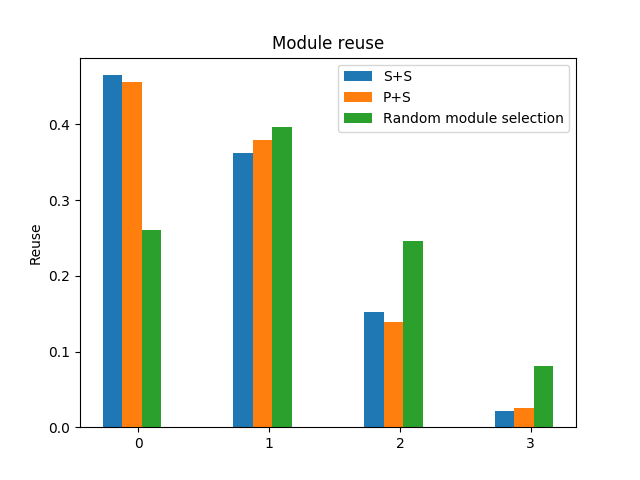
\includegraphics[width=\textwidth]{Chapters/4.Experiments/exp1/figures/600binMNIST_module_reuse_histogram.png}
    \caption{Distribution of module reuse in S+S and P+S searches alongside expected module reuse for random selection of modules in first and second task[green]. This plot is a result of 600 experimental runs.}
    \label{fig:binMNIST.hist}
\end{figure}

For ease of comparison, four plots are automatically generated in both experiments. These visualize the amount of module reuse alongside different metrics such as average training or frequency counts. 
The most intuitive of which is the module reuse bar graph in \ref{fig:binMNIST.hist}. The hypothesis would manifest itself in this plot as a significantly higher blue bar for higher number of reuse compared to the orange bar of P+S. Instead, no difference in reuse for the two scenarios can be seen. Another observation from the figure is that the frequency of modules with no reuse at all is around 66\% higher than the frequency of zero reuse when randomly selecting modules for two paths. This could indicate that training new modules from scratch is simpler for the model than adapting to interface of previously used weights.

These observations differ from our hypothesis that end-to-end training causes confounded interfaces between layers, but this could be caused by the task we are trying to solve being too simple. This again would cause the paths to train very little and the available capacity in the paths to be too high. When the distance in parameter space between initialize parameters and "good enough" parameters are too small, the gain from reusing modules can not be justified. In other words, learning the task \textit{de novo} is simpler than learning the interface-quirks of a preceding previously used module.

\begin{figure}[t]
    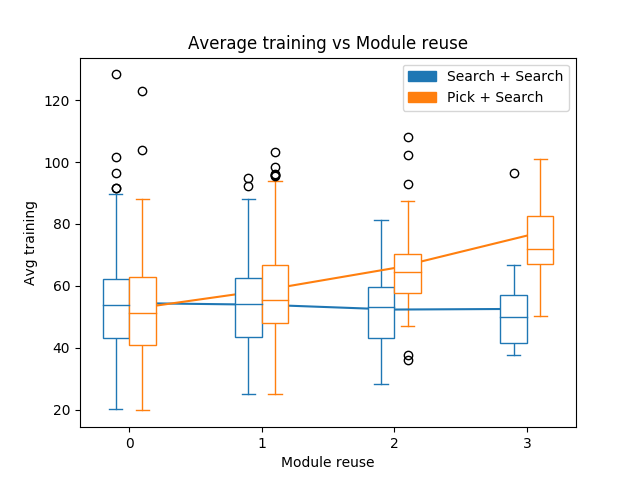
\includegraphics[width=\textwidth]{Chapters/4.Experiments/exp1/figures/600binMNIST_training_boxplot.png}
    \caption{Box-plot depicting average amount of training each module within a path gets for each group of module reuse for both P+S and S+S. }
    \label{fig:binMNIST.box}
\end{figure}

We find support for this claim in \ref{fig:binMNIST.box}, where a clear upwards trend in the average training can be found for P+S, while there does not seem to be a change for S+S. This could mean that in order to reach the same accuracy threshold as S+S, P+S has to undergo more training, meaning the interface between modules is more complicated i P+S than S+S. Please note that the subsets of models with module reuse of 3 is quite small. \ref{fig:binMNIST.hist} visualizes this difference in group size quite well.

The last plot in \ref{fig:binMNIST.layer_reuse} shows something unexpected. The results for search+search and pick+search indicate the same as \ref{fig:binMNIST.hist}, no significant difference in the module reuse. But here, the reuse is shown for each layer in the models. The first layer have significantly lower reuse than the second two. This is the opposite of what we would expect based on the conclusion made by Yosinski et al\cite{yosinski2014transferable}, where the first layers tended to be the most general and easily reusable. This is most likely a property of using multi-layer perceptrons as modules and would disappear if the modules in question consisted of convolutional operations. Fully connected NNs are poor at generalizing to image data because of images complex class manifolds, and as a result of the raw image processing most CNNs end up performing in their first layers, convolutional layers that approximate Gabor-filters ends up being highly transferable.

What we see instead is that most module reuse happens in later layers in the PathNet. It is hard to tell exactly why this is, but a possible explanation is that a path contains more capacity than it needs and the later layers are capable of doing all the heavy lifting. In that case the first layer does not contain use full weights, and therefore there is no incentive to reuse those modules. 

\begin{figure}[t]
    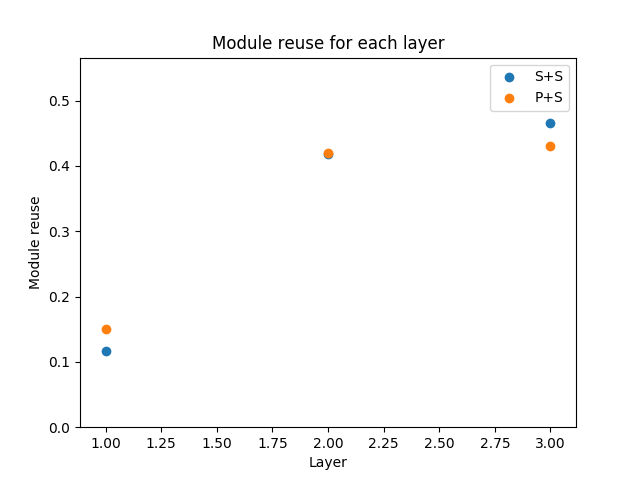
\includegraphics[width=\textwidth]{Chapters/4.Experiments/exp1/figures/600binMNIST_reuse_by_layer.png}
    \caption{This plot shows how the total amount of reuse in all experiments are distributed on the three layers in the PathNet structure }
    \label{fig:binMNIST.layer_reuse}
\end{figure}

Since this implementation is one of fully connected nodes, each neuron have to generalize to its corresponding image pixels, and would therefore be highly task specific. This is the motivation behind performing the quinary MNIST classification experiment in addition to this one. More classes constitute a "harder" classification task, and the change from NNs to CNNs as modules should remove some of the effects we have seen in the plots in this section. Effects we hope to see in Quinary MNIST classification is

\begin{enumerate}
    \item A separation between P+S and S+S in frequency of models with a higher module reuse.
    \item S+S should have a frequency distribution closer to the distribution by randomly choosing modules.
    \item A significantly smaller divergence between P+S and S+S in average training for each module reuse group. 
    \item A more even distribution of module reuse on each layer in a path.
\end{enumerate}


Point 4 because the modules are changed from NNs to CNNs, and 1 through 3 because we increase the task difficulty and therefore also the necessary training time. 

\subsection{Quinary MNIST classification}

\begin{figure}[t]
    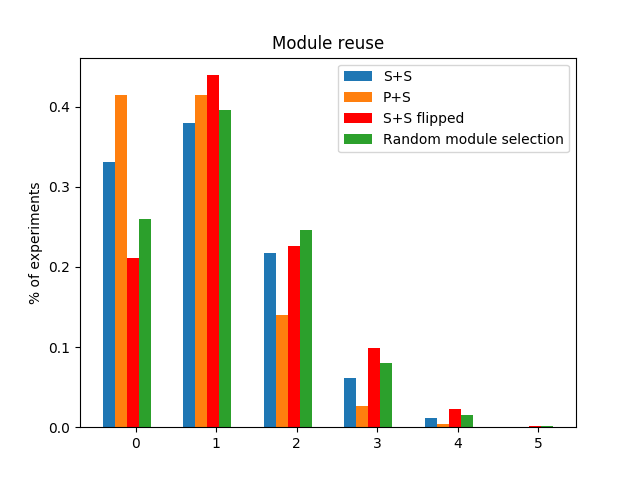
\includegraphics[width=\textwidth]{Chapters/4.Experiments/exp1/figures/535MNIST_module_reuse.png}
    \caption{Frequency histogram equivalent to \ref{fig:binMNIST.hist} for the Quinary MNIST classification experiment. The red bar shows reuse in a training scenario similar to S+S, but where the order of tasks is reversed.}
    \label{fig:quinMNIST.hist}
\end{figure}

\begin{figure}[t]
    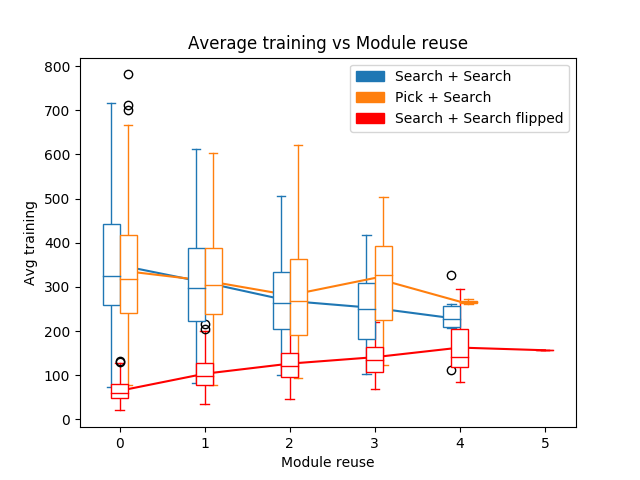
\includegraphics[width=\textwidth]{Chapters/4.Experiments/exp1/figures/535MNIST_training_boxplot.png}
    \caption{Average training box-plot equivalent to \ref{fig:binMNIST.box} except for the addition of a training scenario similar to S+S but where the task order is reversed}
    \label{fig:quinMNIST.box}
\end{figure}

\begin{figure}[t]
    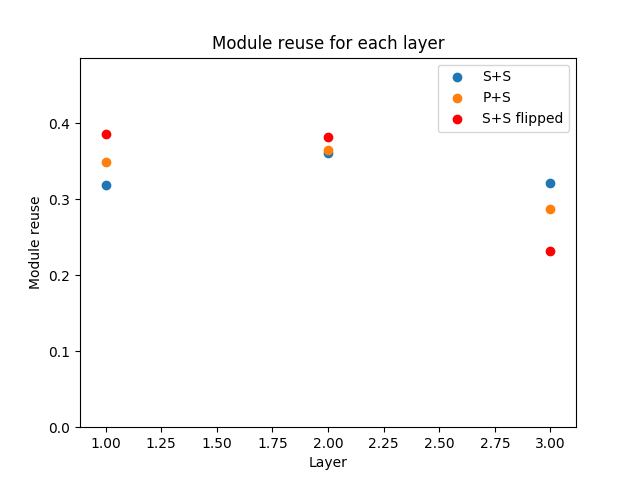
\includegraphics[width=\textwidth]{Chapters/4.Experiments/exp1/figures/535MNIST_reuse_by_layer.png}
    \caption{Frequency of module reuse for each layer in the paths. Equivalent to \ref{fig:binMNIST.layer_reuse} except for the addition of a training scenario similar to S+S but where the task order is reversed}
    \label{fig:quinMNIST.layer_reuse}
\end{figure}


It is quickly eminent from figures \ref{fig:quinMNIST.hist} and \ref{fig:quinMNIST.box} that the increase in task difficulty between binary MNIST and quinary MNIST have uncovered effects predicted in the original hypothesis. In the bar graph \ref{fig:quinMNIST.hist}, the amount of reuse in S+S and P+S have separated, and even though this is not conclusive evidence of the interface confounding predicted, the effect shown here is strong enough to discourage the end-to-end training of a chosen first path. We also see confirmation of point 2 in the list of predictions made in the previous section of this thesis. 

In \ref{fig:quinMNIST.box} the divergence between S+S and P+S for the higher levels of reuse have disappeared, and now a downwards trend in average training is emerging. Recall the point made earlier that the later boxes in this figure represent a significantly smaller group compared to those of less reuse (see \ref{fig:quinMNIST.hist}), but there still looks to be a decline in average training when the amount of reuse within a path increase. This effect can be explained if we suspect the task used for the first path in each experiment to be easier than the second. 

Say task A in a two task system is much simpler than task B. After optimal path for task A have been found and locked, the PathNet will consist of most modules with no training, while those along path A will have a small amount. If task B is harder and more training is done during the search for path B, more reuse of modules means a higher amount of modules in path B have been trained during task A and therefore have received less training in total. The average amount of training for task B will then be lower for higher levels of reuse. 
The opposite will be true if task A is harder than task B. More reuse of modules with more training means the average training for task B will go up for higher levels of reuse. 

The red boxes in figure \ref{fig:quinMNIST.box} confirm this. This part of the plot is from a training scenario similar to Search + Search, but where the order of tasks is reversed\footnote{In S+S, task A consisted of classifying the classes \{0, 1, 2, 3, 4\}, while task B were classes \{5, 6, 7, 8, 9\}}. We see a clear upwards trend in the groupings but also note the average training for each level of module reuse is lower in the flipped S+S scenario.
%WHY!?
In figure \ref{fig:quinMNIST.hist}, the amount of paths with no module reuse in the flipped S+S scenario is half of P+S, which means it has a all around higher module reuse. I previously discussed the fact that the probability of having no reuse is higher for these training scenarios than that of a random module selection, but this is not true for flipped S+S. 
It seems the experiment is simplified by training on the hardest task first. Another experiment should be run to see if this holds true for flipped P+S training.

In figure \ref{fig:quinMNIST.layer_reuse} the difference between S+S and P+S is more significant, and we can also see point 4 in the list of suspected changes confirmed. Reuse is more evenly distributed across the layers. For flipped S+S we can see what we originally expected from this plot, that the level of reuse is higher for the first layers and then decline as the abstraction in each layer increase. 

\section{Conclusion}
In conclusion, results in quinary MNIST classification as well as the comparison with the binary MNIST experiment show promising, if not conclusive, evidence of end-to-end training causing confounded interfaces between modules and a reduction in transferability between task in a multitask scenario. Note should also be taken of how task difficulty effect reuse, and ordering of task from low difficulty and upwards will manifest as a lower average training for paths with a high level of reuse. Results in figure \ref{fig:quinMNIST.hist} tells us there is something undiscovered and unexpected hidden in the ordering of tasks, and further experiments is called for to  uncover this. 

Motivation for these experiments were the possibility of reducing experimentation time by not searching for the first path in the PathNet structure, but the reduction in transferability is dissuading enough to not justify forgoing a full search for all paths. 

